\documentclass[12pt]{article}


\usepackage[dvips,letterpaper,margin=0.75in,bottom=0.5in]{geometry}
\usepackage{cite}
\usepackage{slashed}
\usepackage{graphicx}
\usepackage{amsmath}

\begin{document}
\newcommand{\pt}           {\ensuremath{ p_{\rm T} }}
\newcommand{\Et}           {\ensuremath{ E_{\rm t}     }}

\let\divsymb=\div % rename builtin command \div to \divsymb
\newcommand{\gv}[1]{\ensuremath{\mbox{\boldmath$ #1 $}}} 
\newcommand{\grad}[1]{\gv{\nabla} #1} % for gradient
\renewcommand{\div}[1]{\gv{\nabla} \cdot #1} % for divergence


%\let\vaccent=\v % rename builtin command \v{} to \vaccent{}
%\renewcommand{\v}[1]{\ensuremath{\mathbf{#1}}} % for vectors
%\let\divsymb=\div % rename builtin command \div to \divsymb
%\newcommand{\uv}[1]{\ensuremath{\mathbf{\hat{#1}}}} % for unit vector
\newcommand{\abs}[1]{\left| #1 \right|} % for absolute value
\newcommand{\avg}[1]{\left< #1 \right>} % for average




\let\underdot=\d % rename builtin command \d{} to \underdot{}
\renewcommand{\d}[2]{\frac{d #1}{d #2}} % for derivatives
\newcommand{\dd}[2]{\frac{d^2 #1}{d #2^2}} % for double derivatives
\newcommand{\pd}[2]{\frac{\partial #1}{\partial #2}} % for partial derivatives
\newcommand{\pdd}[2]{\frac{\partial^2 #1}{\partial #2^2}} % for double partial derivatives
\newcommand{\pdc}[3]{\left( \frac{\partial #1}{\partial #2} \right)_{#3}} % for thermodynamic partial derivatives

\newcommand{\planewave}{e^{\textstyle i\vec{k} \cdot \vec{x}}}
\newcommand{\radialwave}{\frac{1}{r} \, e^{\textstyle ikr}} 

\title{Black Body Radiation}
\author{Michael Mulhearn}

\maketitle

\section{Introduction}

A black-body absorbs all incident light waves, regardless of the
frequency or angle of incidence.  It is an idealized model (like a
frictionless surface).  When it is in thermal equilibrium at
temperature $T$, it emits, as we will see, black-body radiation, which
does not depend on the shape or material of the black-body but only
the temperature $T$.

\begin{figure}[thb]
\begin{center}
{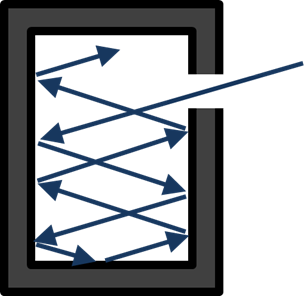
\includegraphics[width=0.35\textwidth]{figs/blackbody.png}}
\end{center}
\caption{\label{fig:blackbody} A model for a blackbody.  Any light waves incident on the hole will be absorbed.}
\end{figure}

Our model for a black body (see Fig.~\ref{fig:blackbody}) is a cube of length $L$ with a small hole
in it.  Light entering the hole will be completely absorbed.  We would
like to understand the frequency spectrum of the emitted radiation.
It turns out that this rather esoteric topic presents an insurmountable problem for the wave theory of light!

\section{Standing Waves in Three Dimensions}

We saw that the Wave Equation in three dimensions is:
\begin{equation}\label{eqn:wave3d}
\frac{1}{c^2} \cdot \pdd{u(x,y,z,t)}{t} = \left( \pdd{}{x} + \pdd{}{y} + \pdd{}{z} \right) u(x,y,z,t) 
\end{equation}  
where we have set v=c because we will only be dealing with light waves in this lecture.

We can guess the 3-D standing wave solution by analogy to the 1-D case
\begin{equation}
u(x,y,z,t) = A \sin(k_x \, x) \sin(k_y \, x) \sin(k_z \, x) \sin( \omega t).
\end{equation}  
This is a solution to wave equation as long as 
\begin{equation}
k^2 \equiv k_x^2 + k_y^2 + k_z^2 = \frac{\omega^2}{c^2}.  
\end{equation}  
The particular standing waves which will have nodes along the sides of the cube of length $L$ will, exactly as in the 1-D case, have wavelengths that are integer fractions of the fundamental wavelength $2L$:
\begin{displaymath}
\lambda_x = \frac{2 L}{n_x}, \; \lambda_y = \frac{2 L}{n_x}, \; \lambda_y = \frac{2 L}{n_z}.
\end{displaymath}
In terms of the wave numbers $k = 2\pi / \lambda$, we have:
\begin{displaymath}
k_x = \frac{\pi n_x}{L}, \; k_y = \frac{\pi n_y}{L}, \; k_z = \frac{\pi n_z}{L}.
\end{displaymath}

\section{Counting Microstates}

For light waves we have:
\begin{displaymath}
k = \frac{2 \pi}{\lambda} = \frac{2 \pi f}{c}
\end{displaymath}
So for the standing waves in the black body we have:
\begin{eqnarray}
\left( \frac{2 \pi f}{c} \right)^2 & = &  k^2 = k_x^2 + k_y^2 + k_z^2 \nonumber \\
& = &  \left( \frac{\pi n_x}{L} \right)^2 + \left( \frac{\pi n_y}{L} \right)^2 + \left( \frac{\pi n_z}{L} \right)^2 \nonumber \label{eqn:densa}\\
\left( \frac{2 L f}{c} \right)^2 & = & n_x^2 + n_y^2 + n_z^2 \equiv n^2
\end{eqnarray}
Where in the last step we have defined $n$ to be the radius in the 3-D space of $(n_x, n_y, n_z)$.  This last step merely says that a particular value of $f^2$ corresponds to a particular value of $n^2$.  We can add to the $n^2$ by various combinations of $n_x$, $n_y$, and $n_z$.

\begin{figure}[thb]
\begin{center}
{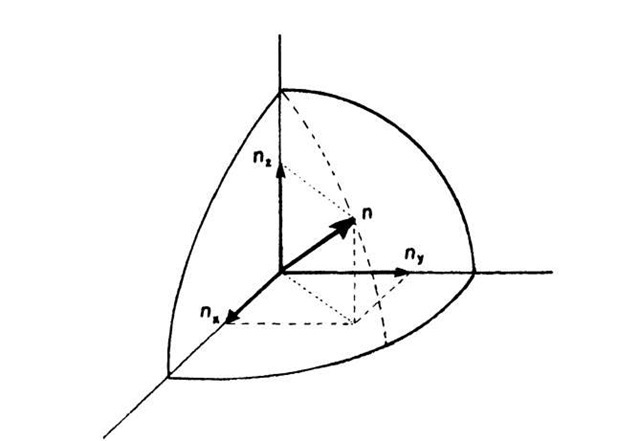
\includegraphics[width=0.35\textwidth]{figs/nspace.jpg}}
\end{center}
\caption{\label{fig:nspace} The states with a particular value of $n$ (corresponding to a particular frequency $f$) will all lie along the sphere $n^2 = n_x^2 + n_y^2 + n_z^2$ }
\end{figure}

To calculate the total number of microstates between $n$ and $n+dn$, we take surface of the sphere shown in Fig.~\ref{fig:nspace} and multiply by the thickness $dn$.   However, since $n_x$, $n_y$, $n_z$ are all positive, we actually only consider $1/8$ of the total area of the sphere.  An additional "feature" of light is that it can have either of two possible "polarizations", so there are in fact two distinct states for every one state we have calculated so far:
\begin{equation}\label{eqn:densb}
dN(n) = \frac{1}{8} \cdot 4 \pi n^2 dn = \frac{\pi}{2} n^2 dn 
\end{equation}
Note that 
\begin{eqnarray*}
k & = &  \frac{\pi n}{L} = \frac{2 \pi f}{c} \\ 
n & = & \frac{2 L f}{c}
\end{eqnarray*}
so we can rewrite Equation~\ref{eqn:densb} as:
\begin{eqnarray}\label{eqn:densc}
dN(f) = \frac{8 \pi f^2 L^3}{c^3} df, \nonumber \\
\frac{dN(f)}{V} = \frac{8 \pi f^2}{c^3} df. 
\end{eqnarray}
This quantity is the number of microstates per unit volume with frequency between $f$ and $f+df$.

%Now suppose that we know the average amount of energy $\bar{E}(f)$ contained by each of these micro %states with frequency $f$.  In terms of the energy density $u$  (the energy per unit unit volume) we have
%\begin{displaymath}
%frac{du}{df} = \frac{\bar{E}(f)}{V} \frac{dN}{df} = \frac{4 \pi f^2}{c^2} \bar{E}(f).
%\end{displaymath}
%t turns out that this $E(f)$ completely breaks classical physics!

\section{Classical Solution}

There is a lot of math in the previous section, but in the end, all we did was count the number of microstates with a frequency between $f$ and $f+df$, to obtain Equation~\ref{eqn:densc}.

Last quarter in Thermodyamics, we derived the energy of an ideal gas
\begin{displaymath}
U = \frac{3}{2} N kT.
\end{displaymath}
We saw that each of the $3N$ degrees of freedom ($x$,$y$, and $z$ momentums for each of the N particles) has an energy $\frac{1}{2}kT$.

The classical solution for the blackbody is quite similar:  we associate $kT$ of energy with each of the microstates that we counted in the previous section.  So the classical prediction for the energy density (energy per unit volume) is

\begin{displaymath}
\frac{du}{df} = kT \times \frac{1}{V} \frac{dN}{df} = \frac{8 \pi f^2}{c^3} kT.
\end{displaymath}
This equation, which spelt the doom of classical physics, is called the "Ultraviolet Catastrophe".  It predicts that most of the energy will be contained within the highest frequency modes.  In fact, if we integrate to find the total energy of the blackbody, we find that the integral diverges.  The classical prediction for a black body is that it contains infinite energy.  Impossible!
 
\section{Planck's Law}

Max Planck proposed a radical (and, as it turned out, correct) solution to the Ultraviolet Catastrophe.  He proposed that energy from the black body could only be emitted in discrete packets of energy, which depend on the frequency as:
\begin{displaymath}
E = h f.
\end{displaymath}
How does this help?  We showed that there are more and more microstates at higher and higher frequencies.  In the wave theory of light, the amplitude of the light wave can be as small as we would like in order to excite all of these many many states.  Since most of them are at very high frequency, we find that most of the energy is at high frequency.  Planck's brilliant solution fixes this with one stroke. Now the higher energy modes come at a higher price in terms of energy.  The Boltzman factor $\exp(-E/kT)$ is now much more costly for the high frequency states.  Problem solved!

To see how this works, we first restrict ourselves to one particular microstate with the particular frequency $f$.  Following Planck's hypothesis, this microstate can have any one of 
\begin{displaymath}
E = 0, hf, 2hf, 3hf, ...
\end{displaymath}
Or equivalently
\begin{displaymath}
E = nhv
\end{displaymath}
for quantum numbers $n=0,1,2,...$  The probability that it will be in the particular micro state with quantum number $n$ is given by the Boltzman factor:
\begin{displaymath}
p(n) = \frac{\exp\left(-\frac{nhf}{kT}\right)}{\sum_n \exp\left(-\frac{nhf}{kT}\right)} 
\end{displaymath}
The average energy of a microstate with frequency $f$ is therefore:
\begin{eqnarray*}
E(f) & = &  \sum_n \; p(n) \, nhf \\
   & = &  \frac{\sum_n nhf \exp\left(-\frac{nhf}{kT}\right)}{\sum_n \exp\left(-\frac{nhf}{kT}\right)} \\
   & = &  hf \cdot \frac{\sum_n nx^n}{\sum_n x^n}
\end{eqnarray*}
where in the last step we have defined
\begin{displaymath}
x = \exp(-hf / kT).
\end{displaymath}
The rest is just a math exercise in series expansion.  Noting that:
\begin{displaymath}
\sum_{n=0}^{+\infty} nx^n = x + 2x^2 + 3x^3 + ... = \frac{x}{1-x}
\end{displaymath}
and
\begin{displaymath}
\sum_{n=0}^{+\infty} x^n = 1+x + x^2 + x^3 + ... = \frac{x}{(1-x)^2}
\end{displaymath}
we obtain
\begin{eqnarray*}
E(f) & = &  hf \frac{x}{1-x} \\
   & = &  hf \frac{1}{1/x-1} \\
   & = & \frac{hf}{\exp(hf/kT)-1}
\end{eqnarray*}
Note that the average energy for a state with frequency $f$ is now suppressed, by the exponential part, at high $f$.

To calculate the energy density we need to multiply this average energy by the number of states per unit volume available with that frequency:
\begin{eqnarray*}
\frac{du}{df} &=& \frac{1}{V} \frac{dN}{df} \times E(f) \\
&=& \frac{8 \pi f^2}{c^3} \times \frac{hf}{\exp(hf/kT)-1} \\
&=& \frac{8 \pi h f^3}{c^3} \frac{1}{\exp(hf/kT)-1}
\end{eqnarray*}
So long Ultraviolet Catastrophe!  The exponential term, which comes from the Boltzman factor, now suppresses the energy density at high frequency.

\begin{figure}[thb]
\begin{center}
{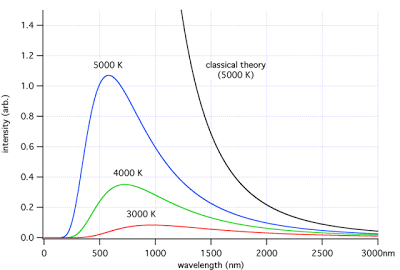
\includegraphics[width=0.55\textwidth]{figs/bbspectrum}}
\end{center}
\caption{\label{fig:nspace} The black body energy spectrum at various temperatures, for the classical and quantum models.  The quantum model is in excellent agreement with experimental results.}
\end{figure}

%\newpage
%\section{Homework Problems}

%\noindent
%{\em Problem 1:} Show that the function:
%\begin{displaymath}
%u(x,y,z,t) = A \cos(k_x \,x + k_y \, y + k_z \, z - \omega t)
%\end{displaymath}
%is a solution to the wave equation.  If we define $k^2 = k_x^2 + k_y^2 + k_z^2$ what is the relation %between $\omega$, $k$, and the characteristic speed from the wave equation $v$?  This is the equation %for a plane wave traveling in an arbitrary direction.

\end{document}




